%Chapter of Implementation
%What my app has, (how it evolved?) in terms of physical structure and technologies involved

\chapter{Implementation}
\label{imple}

\section{Overview}

There are two files in the server, connect.php and add.php. The Arduino makes a post request to the add.php which effectively just calls it and the first thing the add file does is call connect which has the server details and makes creates a connection. Following that there is a SQL query that inserts the values sent in the post request into the appropriate table entries then close the connection. cooodee snippets

The Java Web app details what the server is do when it gets various types of request, be it get or post...(more on requests?). In this type of application you can dynamically printout all the HTML that will be used to make up the page. The usual  HTML, head, body tags are printed at the top and the titles in the table are printed as well. (How it gets the keys?!). The web app uses JDBC to create a driver(idk man) to get the connection to the SQL database. Then using Java language it builds up a SQL query to take out all the values from the database and executes that. This puts all the table entries into a result set and the app cycles through that results set getting the relevant information out. The signed and encrypted hex is encoded as string and some leading zeros are lost in the conversion from byte array to string in the Arduino so these are added now before the string is converted back into a byte array. There is a try catch around the crypto\_box\_open and crypto\_sign\_open method so the server doesn't crash if one result set has been broken. Following this is the conversion from hex into integer for the user to read (how does it do it?) and finally the values are written to the browser along with the ending html tags.


The Due is used in two separate ways in this project; first is the client to the java web app and second is a demonstration of secure public key transmission with another Arduino Uno and Ethernet shield. 

\section{IoT Platform}

The basic concept of this platform is an Arduino Due that takes the current temperature of the room from a DS1820 temperature sensor. Then that data is signed and encrypted with TweetNaCL before being transmitted, using an Ethernet Shield, across to an SQL server. A web application takes the SQL data decrypts, checks the signature is valid then displays on a website. 

graphic here pls


DS1820 is a lost cost temperature sensor that is very accurate, 9 bits of precision and is also low power. It can scavenge power from the data with the arduino and thus does not need it's own power source. 

For the prototype, an Ethernet Shield was used as it is much cheaper than a WiFi shield but ultimately completes the same job. The shield is a simple way to connect arduinos to the internet. The shield used was the second revision, R2 and has a w500 ethernet controller which means it needs an different library to the first revision. Fortunately the two libraries share the same API so the the codes are compatible. Simply swap put the older shield and library and replace with the newer one.


\subsection{Temperature reading}

The DS18S20 temperature sensor is wired up with a pull up 4.7$\Omega$ resistor, between the orange wires, on the bread board shown in figure \ref{fig:tempcircuit}. A pull up resistor is a resistor between the sensor and the positive power supply so that the signal will be a valid logic level if external devices are disconnected or a high impedance is introduced. It is connected to digital pin 9, yellow wire, because it can't be on pins 10, 11, 12, 13 as they will be used by the Ethernet Shield. When looking at the temperature sensor the furtherest left pin is V$_{dd}$ and normally this would be connected to the Arduinos 3.5v or 5v output but the DS18S20 is in parasite power mode which scavenge power off the middle data line, DQ. When the DQ pin is high some of the charge is stored in capacitor DS18S20 to power the device. In parasite power mode both the GND and V$_{dd}$ are connected together, by the blue wire, and then to ground.

\begin{figure}[h]
	\centering
	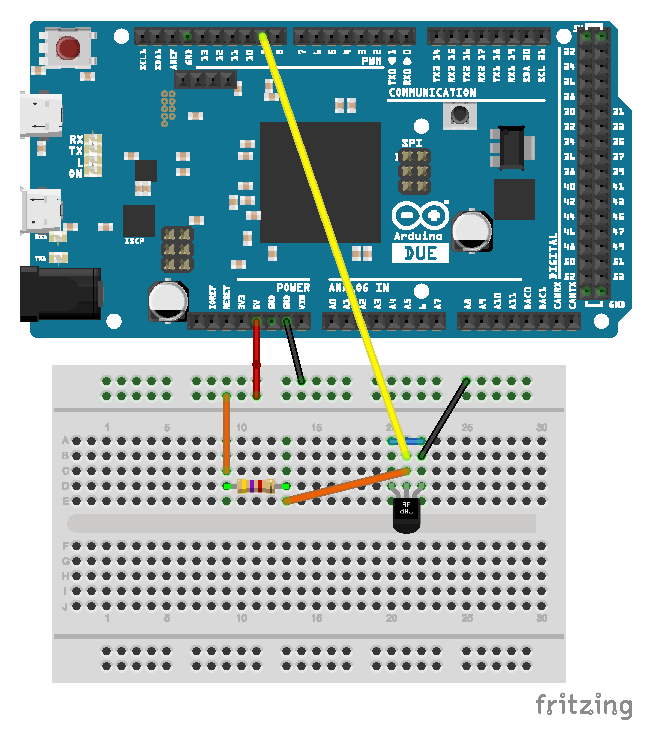
\includegraphics[width=.5\linewidth]{Figures/TempSensor_bb.pdf}
	\caption{DS18S20 in parasitic power mode connected to Arduino}
	\label{fig:tempcircuit}
\end{figure}

%can explain full scratchpad memory, CRC, or hex to int conversion
The library used to read the DS18S20 is OneWire, which is a proprietary library from Maxim. The command \emph{ds.write(0x44, 1)} starts the internal A-D conversion operation. Once this process is finished the data is copied to the Scratchpad registers. A delay is need to charge the capacitor and to ensure conversion is complete before reading the data. Which is done with \emph{ds.write(0xBE)} and then the data is read out using \emph{ds.read()} then put into an array.

\begin{figure}[H]
\begin{lstlisting}[style=Arduino]
  							OneWire  ds(9);
								...
  							ds.write(0x44, 1); 
  						 	delay(1000);

  							present = ds.reset();
  							ds.select(addr);    
 							ds.write(0xBE)

  							Serial.print("  Data = "); 
  							Serial.print(present, HEX);
 						 	Serial.print(" ");
  							for ( i = 0; i < 9; i++) {          
    								data[i] = ds.read();
    								Serial.print(data[i], HEX);
    								Serial.print(" ");
  							}

\end{lstlisting}
\caption{DS18S20 temperature sensor Arduino Code}
\label{snip:tempcode}
\end{figure}


\section{Cryptographic}
\begin{figure}[H]
\begin{lstlisting}[style=Arduino]
#include <TweetNaCl2.h>
TweetNaCl2 tnacl;

byte arduinosk[crypto_box_SECRETKEYBYTES] = {...};
byte arduinosksign[crypto_sign_SECRETKEYBYTES] = {...};
byte serverpk[crypto_box_PUBLICKEYBYTES]  = {...};
byte nonce[crypto_box_NONCEBYTES] = {...};

int const messageLength = crypto_sign_BYTES + 9;
byte message[messageLength] = {...};
unsigned long long signedMessageLength=0;
byte signedCipher[signedMessageLength];
unsigned char signedMessage[messageLength+crypto_sign_BYTES];

tnacl.crypto_sign(signedMessage, &signedMessageLength, message, messageLength, arduinosksign);
tnacl.crypto_box(signedCipher, signedMessage, signedMessageLength, nonce, serverpk, arduinosk);
\end{lstlisting}
\caption{TweetNaCl Arduino Signature and Encryption Code}
\label{snip:nacl}
\end{figure}

The C TweetNaCl has been converted into an Arduino library and therefore needs an instance created called \emph{tnacl}. With this instance the methods needed can be accessed. The keys are preinstalled to avoid the key distribution problem in lines 4-7. The next chunk sets up the messages that are two be passed between the methods. Message is initialised as a byte array of size \emph{messageLength} which can has to be \emph{crypto\_sign\_BYTES}, 32 bytes, plus the message. The first 32 bytes have to be zero for the signing to work. \emph{signedMessage} and \emph{signedMessageLength} are passed in by reference so after \emph{crypto\_sign()} is complete the message with the signature and the size of that array will be in those variables, respectively. The signed message has to have the leading 32 bytes(ummm) be zero but \emph{crypto\_sign()} takes care of that. Now that the plain text message has been signed it is to be encrypted. \emph{signedCipher} and \emph{signedMessage} are passed in by reference as well and the length of the cipher has the same size as the signature. The final product is the signed message cipher and that is the array sent.
%explain what is happening?

\section{Data transmission}
Once the data has been encrypted it is to be packaged up and sent across the network.

\begin{figure}[H]
\begin{lstlisting}[style=Arduino]
#include<Ethernet2.h> //Ethernet Shield R2 library
#include<SPI.h>

byte mac[] = {
0x90, 0xA2, 0xDA, 0x10, 0x2D, 0xD6 //of the Ethernet Shield
};
char server[] = "192.168.0.6"; //IP of apache web server
EthernetClient client;

 if(Ethernet.begin(mac)==0){
      Serial.println("Failed to assign IP");
  }else{
     Serial.println("Assigned IP");
     assigned=1; //static IP?!
  }

if(client.connect(server,80)){
     String data = "temperatureHex=";
     int contentLength = data.length()+final.length();
     Serial.println("Connected");   
     client.println("POST /tempLog/add.php HTTP/1.1"); 
     client.println("HOST: 192.168.0.6"); 
     client.println("Content-Type: application/x-www-form-urlencoded");
     client.print("Content-Length: ");
     client.println(contentLength);
     client.println();
     client.print("temperatureHex=");
     client.print(final);
   }else{
       Serial.println("Failed to Connect");
   }
   
   client.stop();
\end{lstlisting}
\caption{Ethernet interfacing and transmission Code }
\label{snip:ethernet}
\end{figure}
 Just before the cipher is sent the byte array is converted into a String so that it can be passed around easily as one parameter. This is completed simply be cycling through the byte array and adding each entry together. Care has to be taken when there are hexadecimals that are 0x0F or lower. The leading zero is lost during the conversion to String which means the cipher is incorrect and cannot be decrypted. This is solved by explicitly adding an extra ``'0'' String if the byte is less than or equal to 0x0F. First the device needs an IP address which is complete through DHCP by the router, this is completed with the line \emph{Ethernet.begin(mac)} which returns a 1 on successful IP allocation or 0 on failure. If it fails then a static IP can be assigned manually. A connection to the server is attempted using the IP and the port number, 80 in this case. If it successful the information is sent as a POST request, a POST request is a request method in the HTTP protocol. When a server receives a POST request it knows to take the data and complete an action with it. The request makes it known that it wants add.php to be executed upon receiving the data. %extra params, the content size and urlencoding
Once the data is sent the connection can be closed and other actions performed on the Arduino.
 
\section{Server Side}
						%needs an intro
For the prototype, an Apache server, SQL server and Tomcat server were set up using XAMPP on a desktop. The Arduino causes the add.php to be run and the first thing that does is make a connection to the SQL server using SQl server address, username, password and the name of the database. If it can't connect it abandons the task and returns an error message. On successful connect it returns the connection variable.

\begin{figure}[H]
%\begin{lstlisting}[language=PHP]
\begin{lstlisting}[style=PHP]
<?php
   	include("connect.php");
 
   	$link=Connection();
	
	$temp=$_POST["temperatureHex"];
 
	$query = "INSERT INTO tempLog (tempHex) 
		VALUE ('".$temp."')"; 
 
   	mysql_query($query,$link);
   	mysql_close($link);
 
   	header("Location: index.php");
?>
\end{lstlisting}
\caption{Arduino to SQL interfacing code}
\label{snip:php}
\end{figure}

The data to be stored is extracted out of the POST request and place in a variable. Then an SQL query is built up before being sent to the SQL server and the connection terminated. The SQL table contains an ID, the time at which the temperature data was received and the data and is created using the command shown in figure \ref{snip:sql} Notice the corresponding variables, tempLog, the table and tempHex, the data.

\begin{figure}[H]
\begin{lstlisting}[style=SQL]
CREATE TABLE `iotplatform`.`tempLog` ( `id` INT(255) NOT NULL AUTO_INCREMENT , `timeStamp` TIMESTAMP on update CURRENT_TIMESTAMP NOT NULL DEFAULT CURRENT_TIMESTAMP , `tempHex` VARCHAR(100) NOT NULL , PRIMARY KEY (`id`)) ENGINE = InnoDB;
\end{lstlisting}
\caption{SQL database creation code}
\label{snip:sql}
\end{figure}
%InnoDB?
The data stored in the database is still encrypted, now a way is needed to decrypt it and display it to the user. A Java web app, using Java server pages, JSP, was created as there are Java implementations of the TweetNaCl library, among other variations, available \cite{ian}. Eclipse JEE Mars was used to create a dynamic web project which extends HttpServlet for the creation of dynamic web pages. In this you override at least one of the following methods, doGet, doPost, doPut and doDelete so the depending on the type of request received a different action will occur. This application has the code in the doGet as server will receive a get request when it is accessed by a user.

\begin{figure}[H]
\begin{lstlisting}[style=Java]
protected void doGet(HttpServletRequest request, HttpServletResponse response) throws ServletException, IOException {
response.setContentType("text/html");
PrintWriter printWriter  = response.getWriter();
printWriter.println("<html>");
}
\end{lstlisting}
\caption{Prepping the client printer in JSP}
\label{snip:clientprinterjsp}
\end{figure}

The headers and tags you would need and expect in a HTML page can now be print dynamically much like printing to a console. The keys are defined similarly  to the code on the Arduino expect the server has it's own secret key and the Arduino's public key.

\begin{figure}[H]
\begin{lstlisting}[style=Java]
	final String DB_URL="jdbc:mysql://localhost/iotplatform";
	String user = "root"; 
	String password = "";
	try
	        {
	          // Register JDBC driver
	          Class.forName("com.mysql.jdbc.Driver").newInstance();

	            // Open a connection
	            Connection conn = DriverManager.getConnection(DB_URL, user, password);

	            // Execute SQL query
	            Statement stmt = conn.createStatement();
	            String sql;
	            sql = "SELECT id, timeStamp, tempHex FROM tempLog";
	            ResultSet rs = stmt.executeQuery(sql);
	            // Extract data from result set
	            while(rs.next()){
	               //Retrieve by column name
	               int id  = rs.getInt("id");
	               String tempHex = rs.getString("tempHex");
	               Timestamp timeStamp = rs.getTimestamp("timeStamp");
	}
}
\end{lstlisting}
\caption{Accessing the SQL database in JSP}
\label{snip:sqlaccessjsp}
\end{figure}

The app is given the server details and access to it before entering a try catch that prints whatever the error message is to the client. Java database connectivity, JDBC, is an API for client access to a database. The app gets a new instance of JDBC and then opens a connection to the server before building up a query to pull out the contents of the table. The variables are put into a result set which much be accessed for each individually variable with the string name as a parameter. The encrypted message is still in it's String format and needs to be converted back into a byte array. During the conversion to a String on the Arduino half of the leading zeros are lost and they are added before the conversion to byte array. The API in the Java implementation of TweetNaCl is the exact same as the C.

\begin{figure}[H]
\begin{lstlisting}[style=Java]
TweetNaCl.crypto_box_open(signedMessage, cipher, messageLength, nonce, arduinoPublicKey, serverSecretKey);
byte[] javaPlainTextMessage = TweetNaCl.crypto_sign_open(signedCipherArray, ArduinoPublicSignatureKey);
\end{lstlisting}
\caption{Decryption of message and verification of signature in JSP}
\label{snip:decryptjsp}
\end{figure}

The security needs to be taken open in the reverse order as to how it was put on. \emph{TweetNaCl.crypto\_box\_open} passes the decrypted message out by ref but for \emph{TweetNaCl.crypto\_sign\_open} the message without the signature is returned. The variable \emph{javaPlainTextMessage} is the temperature in plain hexadecimal but it still needs conversion to integer so it can be read by the average user. The code is taken from the DS18S20 example.

The web app upon being accessed decrypts and checks the signature of each entry, using the keys that it has stored, in the table before converting the raw hex temperature data into more readable integers and displaying in a simple HTML table that can be accessed by the user. When the Arduino has data to send it will make a POST request to a PHP file on the Apache server which takes the data given to it and places it in the SQL server. (security flaw!)

\section{NaCl}

The TweetNaCl library as it stands in it's original form is not compatible with Arduinos. The C library compiles without errors but the compiler warns that the TweetNaCl method names are undefined and as a result do not perform their tasks. The method simply returns random numbers, it is possibly that it is trying to access some area of memory and simply returns whatever it finds.(ask greg/james). It is not understand why this is the case but it is a simple case of converting the library into C++ syntax. With a header file that has the main methods used in the project and the \#defines and a cpp file with the TweetNaCl code. This is added in the same way to the Arduino IDE and in the code an instance of the class is created and methods are accessed with the dot operator.

The keypair, crypto\_sign, crypto\_box and equivalent opens were used. These are simple to use, abstracted methods that make this library easy to use. For the encryption the method needs the message to be encrypted which needs to have the first 32 bytes be zero, an empty array that needs to be at least the size of the message with the leading zeros, the length of the message, the nonce, arduino public key and the servers private key. This will reveal the temperature data with the signature. To remove the signature, the crypto\_sign\_open method needs the server secret signature key and the signed cipher array.

\section{Machine to Machine}


secure M2M public key transmission
talk more about that

